

%\setcounter{section}{2}
\section{Data Understanding}



\subsection{Gathering Data}
\label{subsec:Gathering Data}
\noindent
The dataset was obtained from \href{https://www.kaggle.com/datasets/austinreese/usa-housing-listings}{Kaggle}. According to the dataset author, the data was scraped from Craigslist in approximately January 2020 and compiled into a single CSV file.

\vspace{6pt}
\noindent
\textbf{Project scope.} This project focuses on rental apartments in the Southern United States (Census Bureau definition: AL, AR, DC, DE, FL, GA, KY, LA, MD, MS, NC, OK, SC, TN, TX, VA, WV). The full dataset spans all 50 states and 12 property types; filtering to the project scope is performed in Phase~3 (Data Preparation). Phase~2 reports below describe the complete collected dataset as obtained from Kaggle.

\subsubsection{Data Requirements}
\noindent
The project required a dataset of US rental housing listings containing: the listing price as the target variable, physical attributes (square footage, bedrooms, bathrooms), amenity flags (pets, smoking, wheelchair access, EV charging, furnished), property type, and geographic identifiers (state, region, latitude, longitude). The data needed to include Southern US states and apartments specifically (the project scope). The selected dataset exceeds these requirements: it covers all 50 states and 12 property types, providing ample records for the Southern-apartment subset.

\subsubsection{Selection Criteria and Data Availability}
\noindent
The raw Kaggle file contains 22 columns across 384,977 rows (558.44 MB). Four text/URL columns (\texttt{id}, \texttt{url}, \texttt{region\_url}, \texttt{image\_url}, \texttt{description}) were excluded from the working dataset, as they carry no predictive signal for price modeling. The remaining 18 columns (four numeric features: \texttt{price}, \texttt{sqfeet}, \texttt{beds}, \texttt{baths}; six binary amenity flags: \texttt{cats\_allowed}, \texttt{dogs\_allowed}, \texttt{smoking\_allowed}, \texttt{wheelchair\_access}, \texttt{electric\_vehicle\_charge}, \texttt{comes\_furnished}; four multi-class categoricals: \texttt{region}, \texttt{type}, \texttt{laundry\_options}, \texttt{parking\_options}; two geographic fields: \texttt{lat}, \texttt{long}; and \texttt{state}) were retained for initial exploration. All further selection decisions are deferred to Task 3.1 (Selecting Data) in Phase~3.

\subsubsection{Tool Compatibility}
\noindent
The dataset was loaded into Python using \texttt{pandas} and \texttt{numpy} without any issues. The CSV format was read directly via \texttt{pandas.read\_csv()} with no encoding errors, parsing failures, or memory constraints (the working file is 37.2 MB). All 18 retained columns were confirmed present and populated upon inspection.

\subsubsection{Issues and Difficulties}
\noindent
No difficulties were encountered during data gathering, access, or loading. Initial inspection revealed the presence of extreme outliers (e.g., maximum price over \$2.7B, maximum square footage over 8.3M), \$0 listings, and missing values in several columns; these issues are documented in Task 2.4 (Verifying Data Quality) and will be addressed during Phase~3 (Data Preparation).


\subsection{Describing Data}
\noindent
The dataset is a single CSV file (comma-separated values) containing 384,977 rows and 18 columns. It holds a mix of numeric, categorical, text, and geographic feature types. The target variable for this project is \texttt{price}.

\begin{table}
    \centering
    \begin{tabular}{||p{2.2cm}|p{5.8cm}|p{6.9cm}||}
    \hline
    \hline
        Feature Type & Features & Notes \\
        \hline
        \hline
        Numeric & price, sqfeet, beds, baths & Target: price. Shows extreme outliers (max \$2.77B, 8.4M sqft). Typical median values: \$1,036, 949 sqft, 2 beds, 1 bath. \\
        \hline
        Categorical (Binary) & cats\_allowed, dogs\_allowed, smoking\_allowed, wheelchair\_access, electric\_vehicle\_charge, comes\_furnished & Boolean amenity flags (0/1). Cats allowed (72.7\%), dogs allowed (70.8\%), and smoking allowed (73.2\%) are permissive; wheelchair access (8.2\%), EV charging (1.3\%), and furnished (4.8\%) are minority features. \\
        \hline
        Categorical (Multi) & region, type, laundry\_options, parking\_options & Multi-class labels. region: 404 Craigslist metro areas; type: 12 property types (apartment, house, townhouse, etc.); laundry\_options: 5 classes; parking\_options: 7 classes. \\
        \hline
        Geographical & lat, long, state & 51 states/territories represented; lat/long coordinates cover the continental US, Alaska, and Hawaii. The project scope (Phase~3) filters to the 17 Southern states. \\
        \hline
    \end{tabular}
    %\caption{Caption}
    %\label{tab:placeholder}
\end{table}

\noindent
The dataset is well-suited for the project's data-mining goals. All required feature categories (physical attributes, amenities, location, price) are present. Issues such as extreme outliers and missing values exist but are documented in Task 2.4 and will be addressed in Phase~3; they do not prevent proceeding.

\subsection{Exploring Data}
\noindent
Exploratory data analysis was conducted using \texttt{df.describe()} in Python (pandas) to compute summary statistics for all numeric and binary features. All figures and statistics in this section describe the full 384,977-row collected dataset (all 50 states, all 12 property types); the Southern-apartment subset is analyzed after scope filtering in Phase~3.

\subsubsection{Summary Statistics}
\noindent
The table below presents descriptive statistics for the numeric features and binary amenity flags. Extreme outliers inflate the mean and standard deviation of \texttt{price} and \texttt{sqfeet}, making the median the more representative central-tendency measure.

\begin{table}[H]
    \centering
    \begin{tabular}{||p{2.8cm}|p{1.8cm}|p{1.8cm}|p{1.8cm}|p{1.7cm}|p{1.7cm}|p{1.7cm}||}
    \hline
    \hline
        Feature & Mean & Std & Min & 25\% & 50\% & 75\% \\
        \hline
        \hline
        price (\$) & 8,826 & 4.46M & 0 & 805 & 1,036 & 1,395 \\
        \hline
        sqfeet & 1,060 & 19,151 & 0 & 750 & 949 & 1,150 \\
        \hline
        beds & 1.91 & 3.49 & 0 & 1 & 2 & 2 \\
        \hline
        baths & 1.48 & 0.62 & 0 & 1 & 1 & 2 \\
        \hline
        lat & 37.23 & 5.55 & -43.53 & 33.45 & 37.65 & 41.14 \\
        \hline
        long & -92.70 & 16.53 & -163.89 & -100.78 & -87.75 & -81.18 \\
        \hline
        \hline
    \end{tabular}
    %\caption{Caption}
    %\label{tab:placeholder}
\end{table}

\vspace{-9pt}

\begin{table}[H]
    \centering
    \begin{tabular}{||p{4.3cm}|p{3cm}|p{3cm}||}
    \hline
    \hline
        Feature & Mean (Proportion) & Interpretation \\
        \hline
        \hline
        cats\_allowed & 0.727 & 72.7\% allow cats \\
        \hline
        dogs\_allowed & 0.708 & 70.8\% allow dogs \\
        \hline
        smoking\_allowed & 0.732 & 73.2\% allow smoking \\
        \hline
        wheelchair\_access & 0.082 & 8.2\% accessible \\
        \hline
        electric\_vehicle\_charge & 0.013 & 1.3\% offer EV charging \\
        \hline
        comes\_furnished & 0.048 & 4.8\% come furnished \\
        \hline
        \hline
    \end{tabular}
    %\caption{Caption}
    %\label{tab:placeholder}
\end{table}

\subsubsection{Numeric Distributions}
\noindent
Price and square footage are heavily right-skewed, with the vast majority of listings concentrated below \$2,000 and 1,500 sq ft respectively. Beds and baths show the expected clustering at integer values, with 1--2 bedrooms and 1 bathroom being the most common configurations.

\begin{figure}[H]
    \centering
    \caption{Exploratory data analysis histograms for key housing variables.}
    \label{fig:EDA}

    \begin{subfigure}[b]{0.489\textwidth}
        \centering
        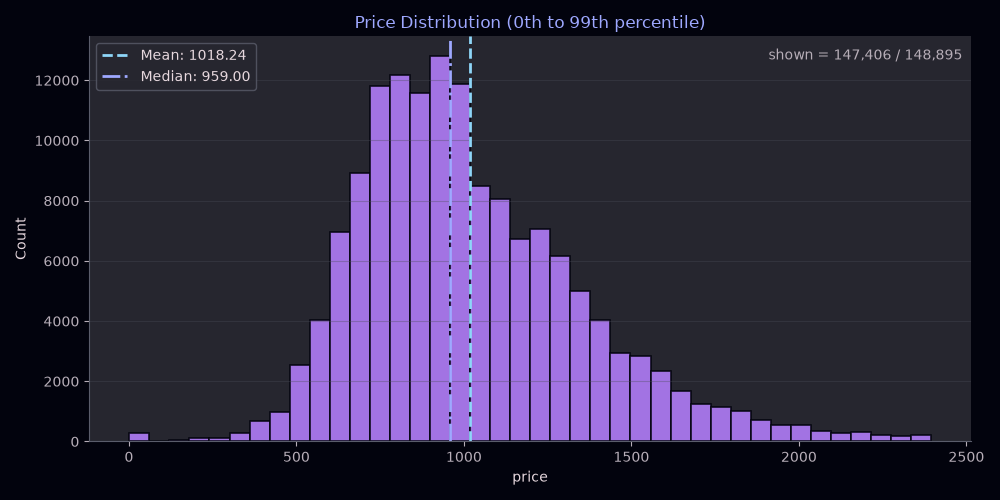
\includegraphics[width=\textwidth]{Assignment/Phase1-5_new/charts/hist_Price Distribution .png}
        \caption{Price distribution}
        \label{fig:EDA_price}
    \end{subfigure}
    \hfill
    \begin{subfigure}[b]{0.489\textwidth}
        \centering
        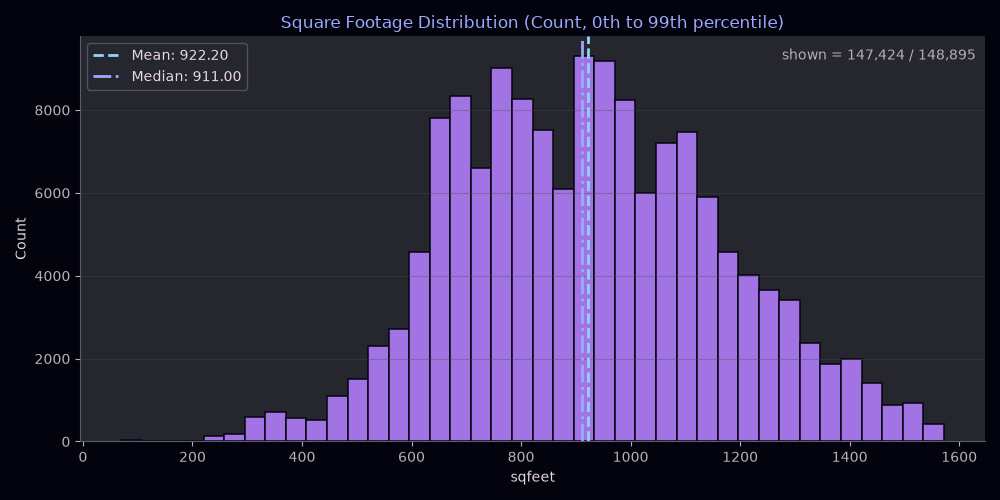
\includegraphics[width=\textwidth]{Assignment/Phase1-5_new/charts/hist_Square Footage Distribution .png}
        \caption{Square footage distribution}
        \label{fig:EDA_sqft}
    \end{subfigure}

    \vspace{-9pt}

    \begin{subfigure}[b]{0.489\textwidth}
        \centering
        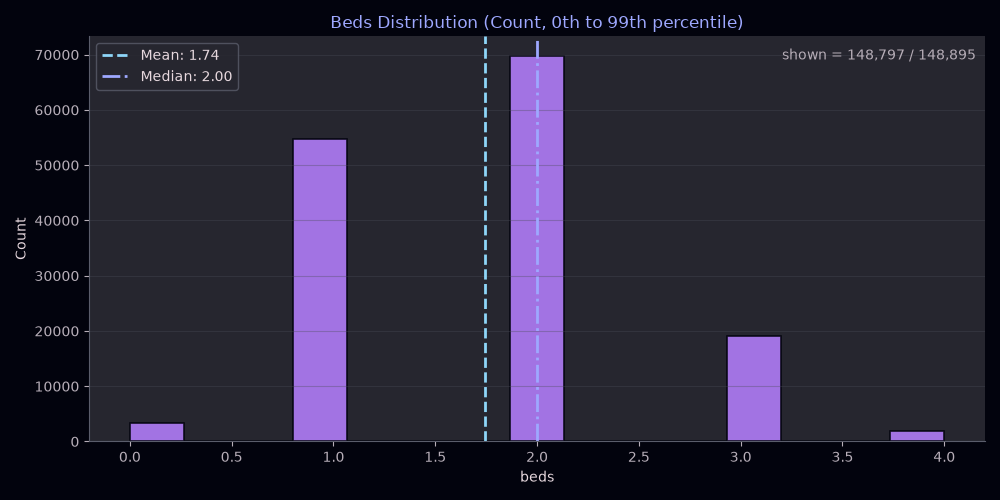
\includegraphics[width=\textwidth]{Assignment/Phase1-5_new/charts/hist_Beds Distribution .png}
        \caption{Beds distribution}
        \label{fig:EDA_beds}
    \end{subfigure}
    \hfill
    \begin{subfigure}[b]{0.489\textwidth}
        \centering
        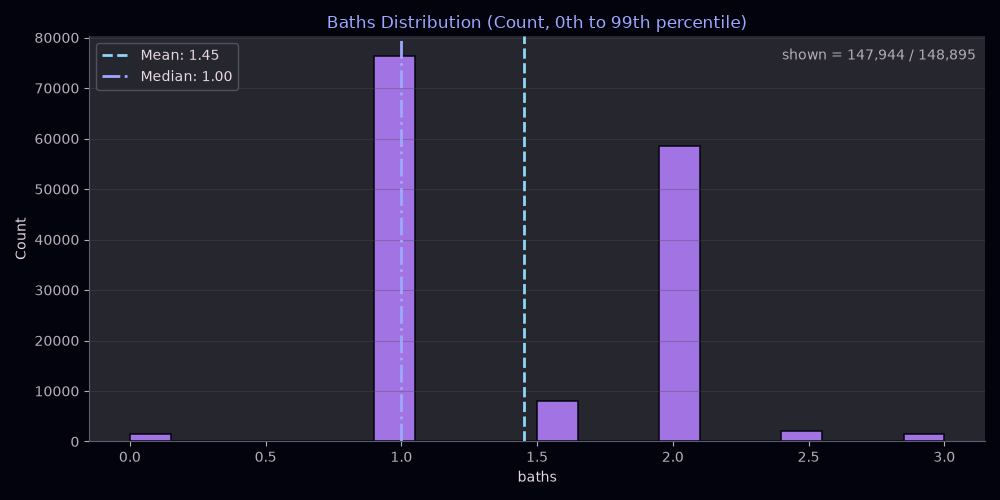
\includegraphics[width=\textwidth]{Assignment/Phase1-5_new/charts/hist_Baths Distribution .png}
        \caption{Baths distribution}
        \label{fig:EDA_baths}
    \end{subfigure}

\end{figure}

\subsubsection{Categorical Distributions}
\noindent
Pie charts for the six binary amenity flags and two multi-class categoricals are shown in Figure~\ref{fig:pie}. Pet and smoking policies skew permissive: 72.7\% of listings allow cats, 70.8\% allow dogs, and 73.2\% allow smoking. Wheelchair access (8.2\%), EV charging (1.3\%), and furnished units (4.8\%) are minority classes. Laundry and parking options show meaningful class imbalance: the most common laundry arrangement (``w/d in unit'') and parking type (``off-street parking'') each account for a plurality of listings, with ``Not Specified'' representing a substantial share in both.

\begin{figure}[H]
    \centering
    \caption{Distribution of selected categorical housing features.}
    \label{fig:pie}

    % Row 1
    \begin{subfigure}[b]{0.329\textwidth}
        \centering
        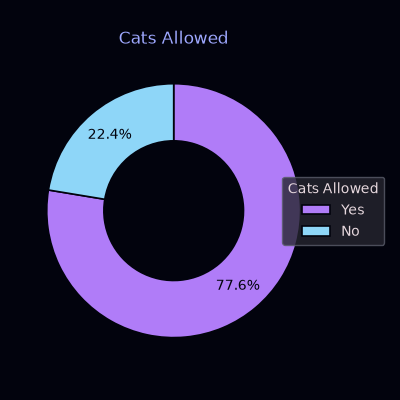
\includegraphics[width=\textwidth]{Assignment/Phase1-5_new/charts/pie_Cats Allowed.png}
        \caption{Cats allowed}
        \label{fig:pie_cats}
    \end{subfigure}
    \hfill
    \begin{subfigure}[b]{0.329\textwidth}
        \centering
        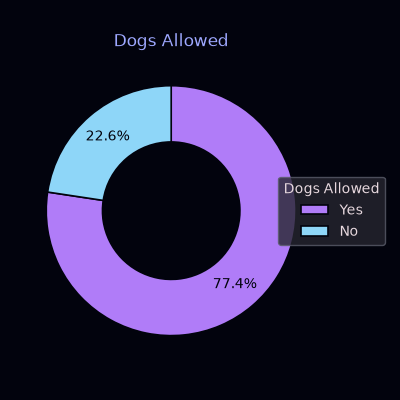
\includegraphics[width=\textwidth]{Assignment/Phase1-5_new/charts/pie_Dogs Allowed.png}
        \caption{Dogs allowed}
        \label{fig:pie_dogs}
    \end{subfigure}
    \hfill
    \begin{subfigure}[b]{0.329\textwidth}
        \centering
        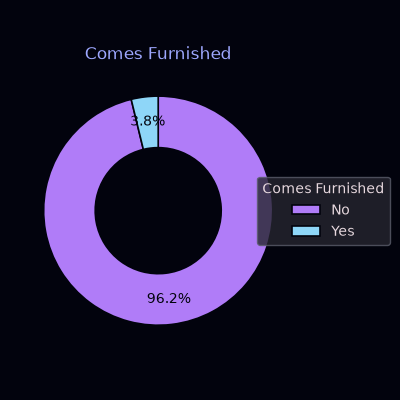
\includegraphics[width=\textwidth]{Assignment/Phase1-5_new/charts/pie_Comes Furnished.png}
        \caption{Comes furnished}
        \label{fig:pie_furnished}
    \end{subfigure}

    \vspace{-9pt}

    % Row 2
    \begin{subfigure}[b]{0.329\textwidth}
        \centering
        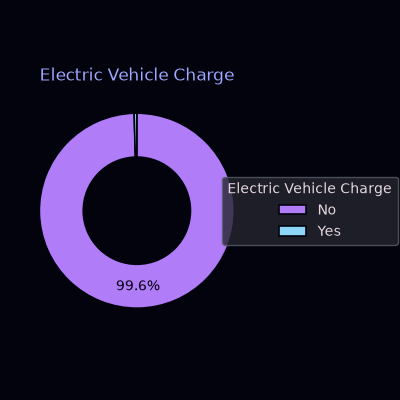
\includegraphics[width=\textwidth]{Assignment/Phase1-5_new/charts/pie_Electric Vehicle Charge.png}
        \caption{Electric vehicle charge}
        \label{fig:pie_ev}
    \end{subfigure}
    \hfill
    \begin{subfigure}[b]{0.329\textwidth}
        \centering
        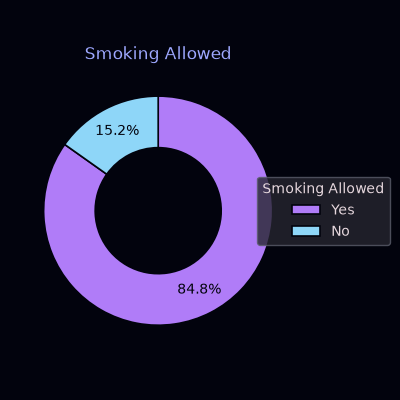
\includegraphics[width=\textwidth]{Assignment/Phase1-5_new/charts/pie_Smoking Allowed.png}
        \caption{Smoking allowed}
        \label{fig:pie_smoking}
    \end{subfigure}
    \hfill
    \begin{subfigure}[b]{0.329\textwidth}
        \centering
        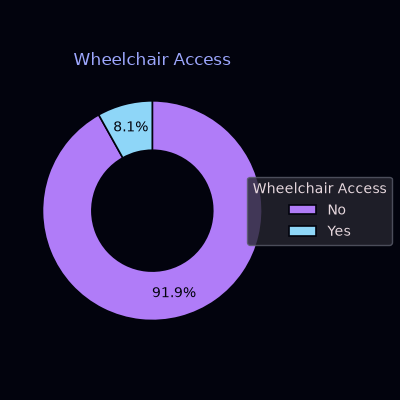
\includegraphics[width=\textwidth]{Assignment/Phase1-5_new/charts/pie_Wheelchair Access.png}
        \caption{Wheelchair access}
        \label{fig:pie_wheelchair}
    \end{subfigure}

    \vspace{-9pt}
    % Row 3
    \begin{subfigure}[b]{0.46\textwidth}
        \centering
        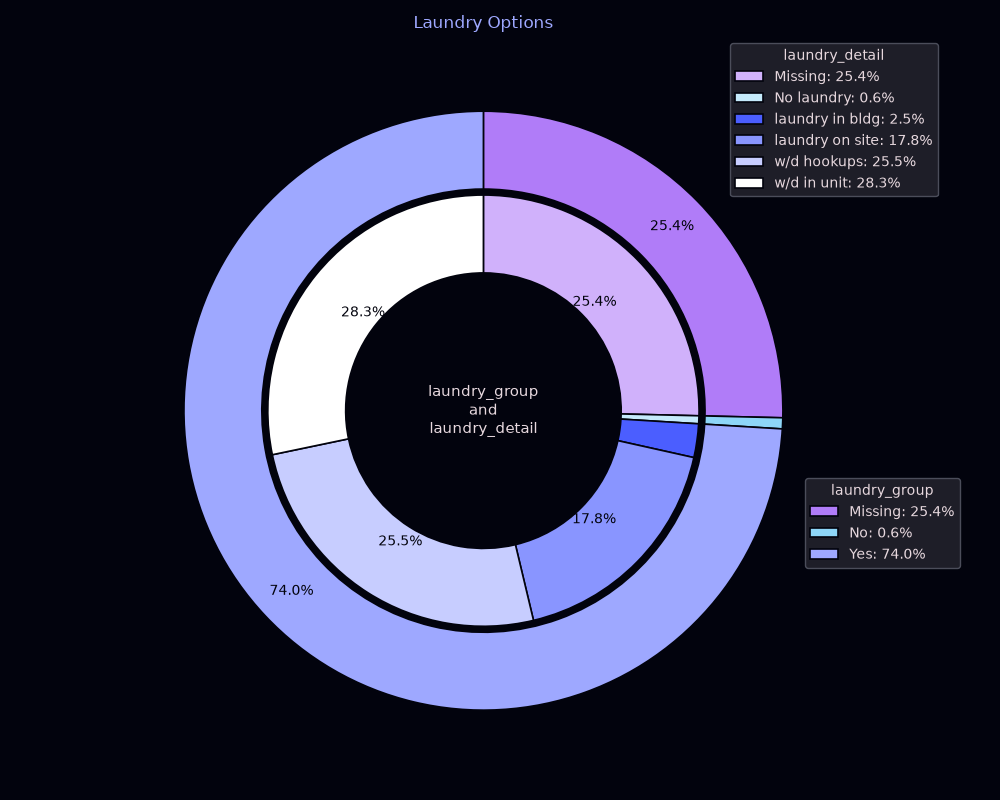
\includegraphics[width=\textwidth]{Assignment/Phase1-5_new/charts/pie_Laundry Options.png}
        \caption{Laundry options}
        \label{fig:pie_laundry}
    \end{subfigure}
    \hfill
    \begin{subfigure}[b]{0.46\textwidth}
        \centering
        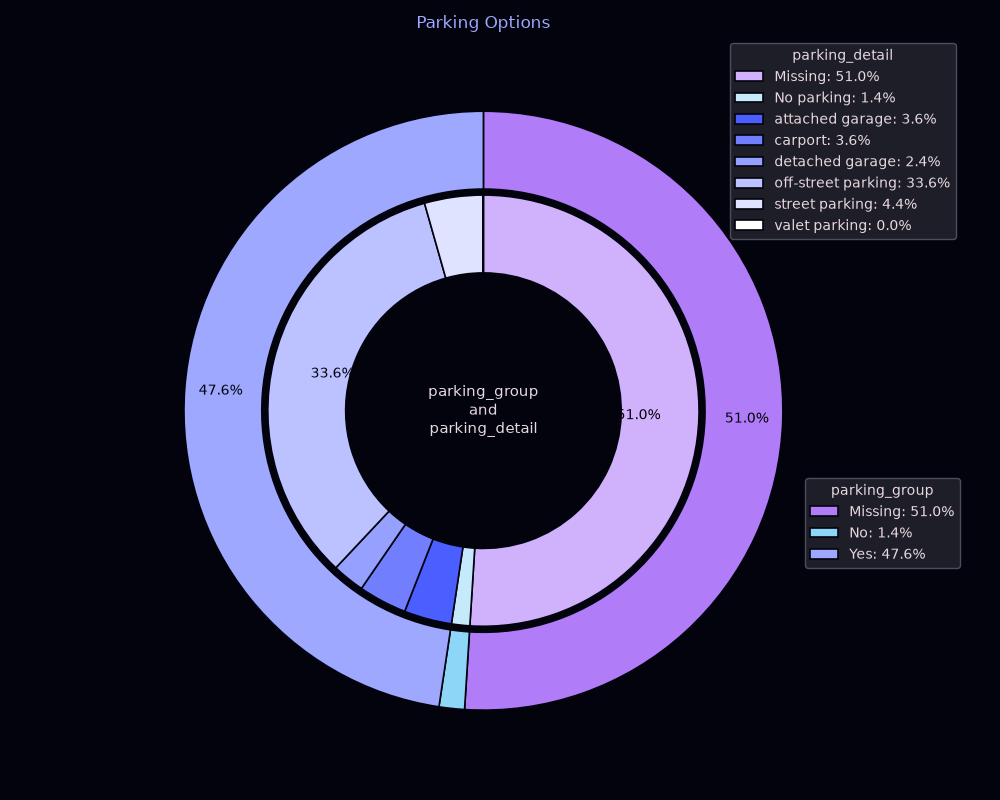
\includegraphics[width=\textwidth]{Assignment/Phase1-5_new/charts/pie_Parking Options.png}
        \caption{Parking options}
        \label{fig:pie_parking}
    \end{subfigure}
\end{figure}

\subsubsection{Correlation Analysis}
\noindent
Pearson and Spearman correlation heatmaps (Figure~\ref{fig:heatmap}) were computed to assess linear and monotonic relationships between each feature and price. Region shows the strongest correlation with price (Pearson $r \approx 0.79$, Spearman $\rho \approx 0.75$), confirming that geographic location is the dominant price driver. State follows (Pearson $r \approx 0.62$, Spearman $\rho \approx 0.61$). Latitude and longitude show negligible linear correlation but a modest Spearman rank correlation, suggesting a non-linear geographic component to pricing.

\begin{figure}[h!]
    \centering
    \caption{Correlation Test - Numeric Features vs Price}
    \label{fig:heatmap}
    \begin{subfigure}[b]{0.49\textwidth}
        \centering
        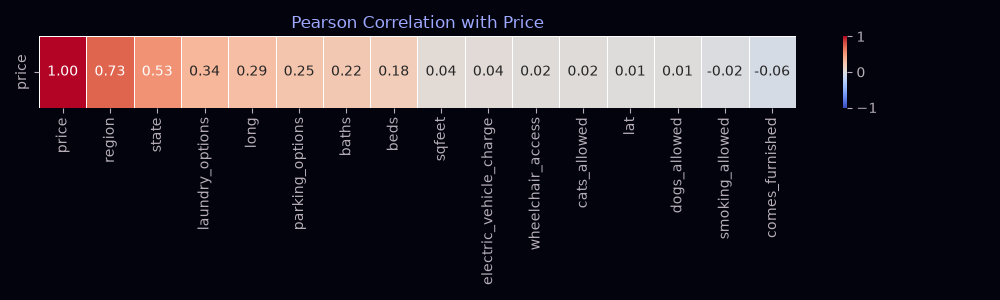
\includegraphics[width=\textwidth]{Assignment/Phase1-5_new/charts/Pearson Correlation with Price.png}
        \caption{Pearson}
        \label{fig:heatmap_Pearson}
    \end{subfigure}
    \hfill
    \begin{subfigure}[b]{0.49\textwidth}
        \centering
        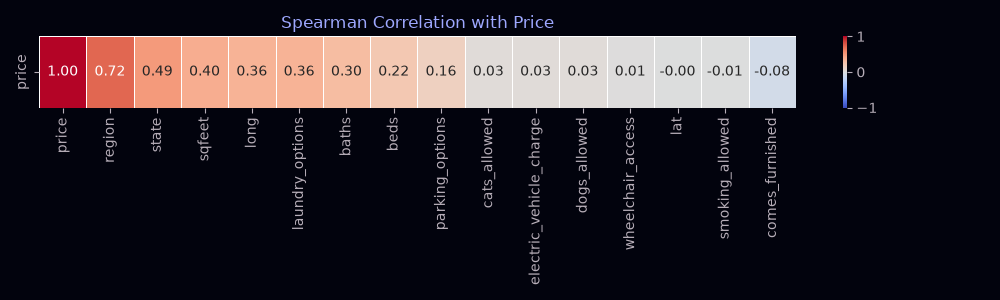
\includegraphics[width=\textwidth]{Assignment/Phase1-5_new/charts/Spearman Correlation with Price.png}
        \caption{Spearman}
        \label{fig:heatmap_Spearman}
    \end{subfigure}
\end{figure}

\subsubsection{Initial Hypotheses}
\vspace{-12pt}
\begin{itemize}[itemsep = -9pt]
    \item Geographic location (region, state) will be the strongest predictors of rental price, consistent with the observed Pearson ($r \approx 0.79$ for region) and Spearman ($\rho \approx 0.75$ for region) correlations.
    \item Square footage will be a meaningful secondary predictor, but weaker than location-based features.
    \item Minority amenity flags (wheelchair access, EV charging, furnished) may have limited predictive power due to severe class imbalance, but their presence may signal premium pricing where they do occur.
\end{itemize}

\subsubsection{Data Quality Signs}
\noindent
Exploration surfaced several data quality concerns that warrant formal verification in Task~2.4:
\vspace{-9pt}
\begin{itemize}[itemsep = -9pt]
    \item Extreme outliers: \texttt{price} reaches \$2.77B and \texttt{sqfeet} reaches 8.39M, orders of magnitude above the 75th percentile. These distort the mean and inflate variance.
    \item Zero-valued listings: 1,307 records have \texttt{price} = \$0 and 48 have \texttt{sqfeet} $<$ 1. These are unlikely to represent genuine rental transactions.
    \item Missing values: \texttt{laundry\_options} and \texttt{parking\_options} are visibly incomplete in the categorical pie charts (the ``Not Specified'' slices), and a small number of lat/long coordinates are absent.
    \item Unrealistic maxima: \texttt{beds} = 1,100 and \texttt{baths} = 75 are implausible for residential rentals and may indicate data-entry errors or non-residential listings.
\end{itemize}


%\newpage

\subsection{Verifying Data Quality}
\label{subsec:Verifying Data Quality}
\noindent
A structured quality assessment was conducted to identify missing values, duplicates, pricing anomalies, and structural issues before data preparation began. Each issue is classified by severity and paired with a proposed remedy.

\subsubsection{Missing Values}
\noindent
All 18 columns in the working dataset were checked for missing values. Four columns contain missing data; the remaining 14 columns (\texttt{id}, \texttt{region}, \texttt{price}, \texttt{type}, \texttt{sqfeet}, \texttt{beds}, \texttt{baths}, \texttt{cats\_allowed}, \texttt{dogs\_allowed}, \texttt{smoking\_allowed}, \texttt{wheelchair\_access}, \texttt{electric\_vehicle\_charge}, \texttt{comes\_furnished}, \texttt{state}) are complete with 0\% missing.

\begin{table}[H]
    \centering
    \begin{tabular}{||p{3cm}|p{2.5cm}|p{2cm}|p{2.5cm}|p{4cm}||}
    \hline
    \hline
        Feature	& Missing Count & Missing \% & Severity & Proposed Remedy \\
        \hline
        \hline
        parking\_options	& 140,687	& 36.54\% & Major & Create ``Not Specified'' category to preserve all records \\
        \hline
        laundry\_options	& 79,026	& 20.53\% & Major & Create ``Not Specified'' category to preserve all records \\
        \hline
        lat	& 1,918	& 0.50\% & Minor & Drop rows; geographic imputation is unreliable across 404 regions \\
        \hline
        long	& 1,918	& 0.50\% & Minor & Drop rows; same rows as missing lat \\
        \hline
        \hline
    \end{tabular}
    %\caption{Caption}
    %\label{tab:placeholder}
\end{table}

\subsubsection{Duplicate Rows}
\noindent
A full duplicate-row check was performed across all 18 columns of the working dataset. No duplicate rows were found among the 384,977 records, confirming each listing is unique.

\subsubsection{Anomalies and Outliers}
\vspace{-12pt}
\begin{itemize}[itemsep = -9pt]
    \item \textbf{\$0 listings} (1,307 records, 0.34\% of data): These may represent listings open to negotiation but introduce noise into price modeling. \textbf{Severity: Minor.} \textbf{Remedy:} Remove these records, as \$0 cannot represent a genuine rental price and would distort regression training.
    \item \textbf{Sub-1 sq ft listings} (48 records, 0.01\% of data): Physically impossible as habitable rental space. \textbf{Severity: Minor.} \textbf{Remedy:} Remove these records.
    \item \textbf{Extreme price outliers} (94 records above \$100K, plus a maximum of \$2.77B): These fall far outside the interquartile range and inflate the dataset mean to \$8,826 vs.\ a median of \$1,036. \textbf{Severity: Moderate.} \textbf{Remedy:} Apply percentile-based capping or IQR-based filtering during Phase~3 cleaning to retain the bulk of the distribution while removing extreme tails.
    \item \textbf{Extreme square footage outliers} (82 records above 10,000 sq ft, plus a maximum of 8.39M sq ft): Analogous to price extremes. \textbf{Severity: Moderate.} \textbf{Remedy:} Same percentile- or IQR-based approach as price outliers.
    \item \textbf{Unrealistic bed/bath counts} (beds $\leq$ 0: 10,978 records; baths $\leq$ 0: 3,107 records; beds $>$ 20: 4 records; baths $>$ 10: 4 records): Bedrooms or bathrooms at 0 are plausible (studio apartments, land rentals), but values exceeding 20 beds or 10 baths are implausible for residential rentals. \textbf{Severity: Minor.} \textbf{Remedy:} Retain 0-bedroom and 0-bathroom records (valid studio/land listings); cap or remove records with beds $>$ 20 or baths $>$ 10.
\end{itemize}

\subsubsection{Overall Quality Verdict}
\noindent
The dataset is of sufficient quality to proceed to Phase~3 (Data Preparation), provided the remedies outlined above are applied. The two most impactful issues are (1) the 36.54\% missing rate in \texttt{parking\_options}, which can be preserved via a ``Not Specified'' level rather than through deletion, and (2) extreme price/square-footage outliers that would distort model training if left untreated. No data collection rework is required.




